\begin{figure}[H]
  \centerline{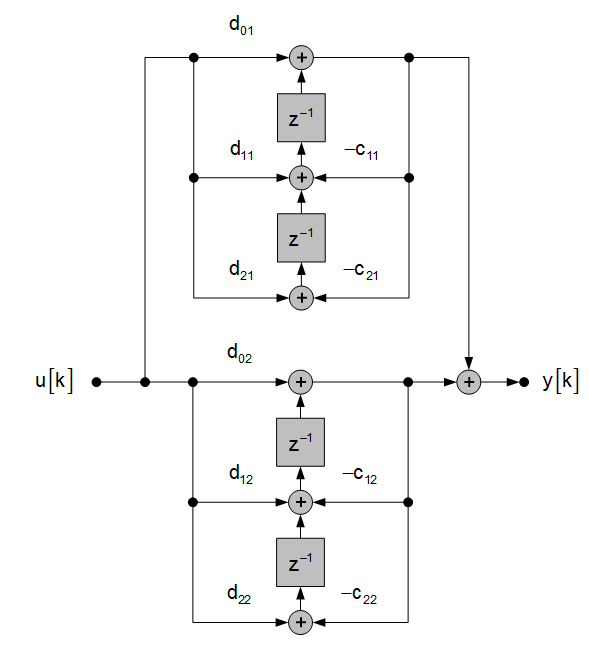
\includegraphics[width=0.6\textwidth]{SignalflussParallelstruktur.png}}
\end{figure}

\noindent \bigskip

\centerline  {\fontfamily{phv}\fontsize{50}{60}\selectfont Systemtheorie Teil B} 

\noindent \medskip

\centerline  {\fontfamily{phv}\fontsize{23}{30}\selectfont  - Zeitdiskrete Signale und Systeme -}

\noindent \bigskip
\noindent \bigskip

\centerline  {\fontfamily{phv}\fontsize{23}{30}\selectfont  Manfred Strohrmann}\medskip

\noindent 

\centerline  {\fontfamily{phv}\fontsize{23}{30}\selectfont Urban Brunner}

\vspace{6.0\baselineskip}

\begin{figure}[H]
  \centerline{
\includegraphics[width=0.6\textwidth]{FH_Logo.png}}
\end{figure}

\clearpage